% This file was created by tikzplotlib v0.9.8.
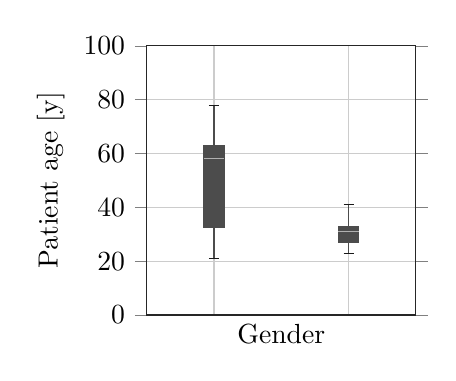
\begin{tikzpicture}

\begin{axis}[
axis line style={white!15!black},
height=5cm,
tick align=outside,
width=5cm,
x grid style={white!80!black},
xlabel={Gender},
xmajorgrids,
xmajorticks=false,
xmin=0.5, xmax=2.5,
%xtick style={color=white!15!black},
xtick={1,2},
xticklabels={F(39),M(15)},
y grid style={white!80!black},
ylabel={Patient age [y]},
ymajorgrids,
%ymajorticks=false,
ymin=0, ymax=100,
%ytick style={color=white!15!black}
]
\addplot [white!29.8039215686275!black, opacity=1]
table {%
1 32.5
1 21
};
\addplot [white!29.8039215686275!black, opacity=1]
table {%
1 62.7652292950034
1 77.6673511293635
};
\addplot [white!10!black, opacity=1]
table {%
0.9625 21
1.0375 21
};
\addplot [white!10!black, opacity=1]
table {%
0.9625 77.6673511293635
1.0375 77.6673511293635
};
\addplot [white!29.8039215686275!black, opacity=1]
table {%
2 27
2 23
};
\addplot [white!29.8039215686275!black, opacity=1]
table {%
2 33
2 41
};
\addplot [white!10!black, opacity=1]
table {%
1.9625 23
2.0375 23
};
\addplot [white!10!black, opacity=1]
table {%
1.9625 41
2.0375 41
};
\path [draw=white!29.8039215686275!black, fill=white!29.8039215686275!black]
(axis cs:0.925,32.5)
--(axis cs:1.075,32.5)
--(axis cs:1.075,62.7652292950034)
--(axis cs:0.925,62.7652292950034)
--(axis cs:0.925,32.5)
--cycle;
\path [draw=white!29.8039215686275!black, fill=white!29.8039215686275!black]
(axis cs:1.925,27)
--(axis cs:2.075,27)
--(axis cs:2.075,33)
--(axis cs:1.925,33)
--(axis cs:1.925,27)
--cycle;
\addplot [white!69.0196078431373!black, opacity=1]
table {%
0.925 58.2888432580424
1.075 58.2888432580424
};
\addplot [white!69.0196078431373!black, opacity=1]
table {%
1.925 31
2.075 31
};
\end{axis}

\end{tikzpicture}
